\documentclass[11pt, a4paper, oneside]{article}

\usepackage{indentfirst}

% hifenização e outras especificações para português
\usepackage[portuguese]{babel}
\usepackage{listings}
% para ter imagens, depois define a directoria de imagens
\usepackage{graphicx}
\graphicspath{{./imagens/}}
\usepackage[utf8]{inputenc}    

\usepackage{listings}
\usepackage{color}
 
\definecolor{dkgreen}{rgb}{0,0.6,0}
\definecolor{gray}{rgb}{0.5,0.5,0.5}
\definecolor{mauve}{rgb}{0.58,0,0.82}
\usepackage{color}
\usepackage{listings}
\lstset{ %
language=C++,                % choose the language of the code
basicstyle=\footnotesize,       % the size of the fonts that are used for the code
numbers=left,                   % where to put the line-numbers
numberstyle=\footnotesize,      % the size of the fonts that are used for the line-numbers
numberstyle=\tiny,
stepnumber=1,                   % the step between two line-numbers. If it is 1 each line will be numbered
numbersep=5pt,                  % how far the line-numbers are from the code
keywordstyle=\color[rgb]{0,0,1},
basicstyle=\tiny,
commentstyle=\color[rgb]{0.133,0.545,0.133},
stringstyle=\color[rgb]{0.627,0.126,0.941},
showspaces=false,               % show spaces adding particular underscores
showstringspaces=false,         % underline spaces within strings
showtabs=false,                 % show tabs within strings adding particular underscores
frame=single,           % adds a frame around the code
tabsize=2,          % sets default tabsize to 2 spaces
captionpos=b,           % sets the caption-position to bottom
breaklines=true,        % sets automatic line breaking
breakatwhitespace=false,    % sets if automatic breaks should only happen at whitespace
escapeinside={\%*}{*)}          % if you want to add a comment within your code
}

% hiperligações
\usepackage{hyperref}
\hypersetup{colorlinks=true, urlcolor=blue, linkcolor=black}

% escrever acentos e coisas do género sem que o latex se desoriente
\usepackage[utf8]{inputenc}

% para ter imagens, depois define a directoria de imagens
\usepackage{graphicx}
\graphicspath{{./imagens/}}

\usepackage[labelformat=simple]{caption}
\usepackage[labelformat=empty]{subcaption}

% para ter a informação de quantas páginas tem o documento
\usepackage{lastpage}

% definir o cabeçalho e rodapé
\usepackage{fancyhdr}
\pagestyle{fancy}
\fancyhead[L]{\small{Gestão de Campeonatos de Orientação}}
\fancyhead[R]{\small{Processamento de Linguagens}}

% ter enumerações alinhadas
\usepackage{enumitem}

% escrever algoritmos
\usepackage[algoruled]{algorithm2e}

% definir comandos especiais
\newcommand\doubleplus{+\kern-1.3ex+\kern0.8ex} %

\newcommand{\todo}[1] {\textcolor{BrickRed}{\begin{quote}#1\end{quote}}}

%\usepackage{listings}


%%%%%%%%%%%%%%%%%%%%%%%%%%%%%%%%%%%%%%%%%%%%%%
%% inicio do documento
\begin{document}
\title{Gestão de Campeonatos de Orientação}
\date{\today\\Universidade do Minho}
\author{
  Bruno Ferreira\\
  {\small A61055}\\
  \and
  Cláudia Oliveira\\
  {\small A60987}\\
  \and
  Vanessa Campos\\
  {\small A54801}\\
}

\maketitle

\begin{figure}[h]
\begin{center}

\includegraphics[width=0.4\linewidth]{logo}
\end{center}
\end{figure}


\begin{abstract}

  O presente trabalho foi desenvolvido no âmbito da Unidade Curricular de Processamento de Linguagens e tem como principal objetivo o aumento da experiência na Linguagem Imperativa C, a capacidade de escrever gramáticas independentes de contexto que satisfaçam a condição de LR(), a utilização de compiladores como o lex/yacc e o desenvolvimento de processadores de linguagem. Ao longo deste relatório iremos explicar as estruturas de dados que foram implementadas para o desenvolvimento deste trabalho, bem como todas as decisões que foram tomadas.

\end{abstract}
\newpage

\tableofcontents
\listoffigures 

\newpage
\section{Introdução}
A Orientação é um desporto que tem como objetivo percorrer uma determinada distância, onde o atleta tem de obrigatoriamente passar pelos pontos que estão indicados no mapa que lhe é atribuído.

Neste contexto temos a gestão de campeonatos de orientação onde é necessário saber a informação das provas que são efetuadas, os participantes envolvidos e os tempos que cada um obteve de modo a serem obtidas as classificações necessárias.
O objetivo principal é a leitura de ficheiros onde estes tem uma configuração definida pelo ficheiro de configuração e depois a leitura do CSV com a informação dos jogadores e mais tarde o geramento de um página HTML onde é apresentada a informação tratada.

Para a implementação foi necessário a construção de gramáticas independentes de contexto, implementação de parses para cada ficheiro que necessário, e a utilização do lex e yacc para retirar a informação necessária.


\newpage
\section{Desenvolvimento}

\subsection{Contextualização do Problema}

Flex é uma ferramenta para gerar automaticamente analisadores léxicos, isto é, programas que reconhecem padrões léxicos num texto. O Flex é uma evolução da ferramenta Lex, mas com a caraterística de ser mais rápido que este (Fast Lex).

Yacc é utilizado para sistemas operacionais Unix, onde o seu principal objetivo e gerar analisadores sintáticos. No entanto o yacc tem de ser utilizado em conjunto com o lex, pois o yacc não consegue ler a partir de uma entrada de dados, daí a utilização  do lex para que este gere os tokens que mais tarde são usados pelo yacc para o processamento.

Gramática Independentes de contexto é uma gramática formal onde são definidas regras de produção da 
 V $\rightarrow$ W onde V é um símbolo não terminal e w um conjunto de símbolos terminais ou variáveis (W no entanto também pode ser nulo).

\subsection{Gestão de Campeonatos de Orientação }

Neste segundo trabalho de Processamento de Linguagens foi-nos proposto a seleção de um projeto entre vários propostos. Após uma análise e chegada a uma concordância, o nosso grupo optou por escolher o tema de Gestão de Campeonato de Orientação.

Com este enunciado tem-se que existem várias operações que ocorrem em simultâneo, pois existe os ficheiros:
\begin{itemize}
\item Ficheiro de Resultados é um ficheiro CSV, onde são guardados os resultados obtidos em cada prova.

\item Ficheiro de Configuração é um ficheiro que vai definir o processamento a realizar, isto é quais as provas e os campos que vão ser tratados
\end{itemize}


\subsection{Enunciado}

De uma maneira geral, para este trabalho pretende-se desenvolver os seguintes pontos:

\begin{itemize}
\item Especificação de uma gramática para a linguagem de comandos da consola;
\item Especificação de uma gramática para a linguagem de especificação de connfigurações;
\item Especificação de uma gramática para os ficheiros de resultados;
\item Desenvolver os respetivos parses;
\item Adicionar as ações semânticas necessárias,
\end{itemize}


\subsection{Descrição do Problema}

Utilizando o flex, yac e gramáticas independentes de contexto era necessário a desenvolvimento de uma aplicação, que permita o tratamento de ficheiros e gere o HTML como os resultados pretendidos.

No entanto existem requisitos consoante ao funcionamento da aplicação. Esta deve possuir um ambiente de consola e implementar os seguintes comandos:
\begin{itemize}
\item Carregar configuração - Permite carregar o ficheiro de configuração;
\item Carregar base de dados - Carregar um ficheiro de dados previamente guardado;
\item Carregar resultado de prova - Carregar o ficheiro de resultados;
\item Calcular Ranking - Permnite calcular o ranking de pontuação dos atletas;
\item Gravar base de dados - Guardar a informação que existem na memória num ficheiro;
\item Sar -  Termina a aplicação.
\end{itemize}

É a partir daqui que os ficheiro de resultados e configuração são lidos e depois as operações são executadas. 

Antes de ser criado o HTML a aplicação tem de ser configurada.
A informação para tal é lida de um ficheiro de configuração onde nele são definidos os campos:
\begin{itemize}
\item Titulo - Titulo da prova em causa;
\item nporvas - nº de provas a realizar;
\item N - Indicados do topN ;
\item campos - Ordem dos campos quando no CSV;
\item score - Pontuação obtida;
\end{itemize}




\newpage

\section{Desenvolvimento do Programa}
Como este projeto implica muito o tratamento de de diferentes aspetos, foi decidido estruturar-se o projeto consoante as  funções que cada ficheiro implica.

\subsection{Estrutura de Dados}
Para a criação das estruturas de dados, foi usado a ferramenta \textit{gabs} disponibilizada pelo professor que cria a estrutura e os seus construtores quando é executada com uma gramática abstrata com argumento.

De modo a utiliza-se a ferramenta era necessário a criação de uma gramática abstrata que depois iria ser passada aos gabs.

Abaixo será apresentado um exemplo da implementação, no entanto em \ref{sec:Anexos} Anexos  puderam ser consultadas as restantes gramáticas abstratas.

A gramática a apresentar é a usada para o ficheiro de configuração. Assim sendo tem-se:
\begin{lstlisting}[language=C, caption={Gramática Abstrata Para o Ficheiro de configuração}]
<ga>
  Confs -> cons_cfg_Confs(Conf Confs)
        |  cons_cfg_Confs_NIL()
        ;

  Conf -> cons_cfg_Conf_Titulo(STR)
       |  cons_cfg_Conf_Nprovas(INT)
       |  cons_cfg_Conf_Ntop(INT)
       |  cons_cfg_Conf_Campos(Lcampos)
       |  cons_cfg_Conf_Tempo(INT)
       |  cons_cfg_Conf_Chave(INT)
       |  cons_cfg_Conf_Nome(INT)
       ;

  Lcampos -> cons_cfg_Lcampos_Lcampos(Lcampos INT)
          |  cons_cfg_Lcampos_Campo(INT)
          ;
</ga>
\end{lstlisting}

A estrutura que é gerada para o armazenamento dos campos que a gramática abstrata definiu, é divida consoante o nível em que estamos, isto é, nós começamos por ter a estrtura que vai abragir mais campos, neste caso o total de configurações, depois temos o que é um configuração e por último a estrutura que vai guardar um para uma configuração.

\begin{lstlisting}[language=C, caption={Estrutura de dados para armazenar as configurações}]
struct sConfs 
{ int flag;
  union {  
    struct {
        Conf s1;
        Confs s2;
      } d1;
    struct {
      } d2;

  } u;
};
\end{lstlisting}

\newpage

\begin{lstlisting}[language=C, caption={Estrutura de dados que armazena uma configuração }]
struct sConf 
{ int flag;
  union {  
    struct {
        char * s1;
      } d1;
    struct {
        int s1;
      } d2;
    struct {
        int s1;
      } d3;
    struct {
        Lcampos s1;
      } d4;
    struct {
        int s1;
      } d5;

  } u;
};
\end{lstlisting}

\begin{lstlisting}[language=C, caption={Estrtutura de dados que armazena os campos de um configuração}]
struct sLcampos 
{ int flag;
  union {  
    struct {
        Lcampos s1;
        int s2;
      } d1;
    struct {
        int s1;
      } d2;

  } u;
};
\end{lstlisting}

Onde se tem que cada struct acima apresentada deriva de cada uma das produções que foram indicadas em na gramática abstrata.


\subsection{Asinatura das Funções Utilizadas}
Vamos agora apresentar as assinaturas das funções que foram utilizadas para nós dar suporte à implementação do nosso projecto.

Quando falamos das funções temos: 
\begin{lstlisting}[language=C, caption={Construtores do Fihceiro de Configuração}]
/* -----------------------------------
 * Constructor Function Signatures
 * -----------------------------------
 */

Confs  cons_cfg_Confs( Conf a1, Confs a2);
Confs  cons_cfg_Confs_NIL();

Conf  cons_cfg_Conf_Titulo( char * a1);
Conf  cons_cfg_Conf_Nprovas( int a1);
Conf  cons_cfg_Conf_Ntop( int a1);
Conf  cons_cfg_Conf_Campos( Lcampos a1);
Conf  cons_cfg_Conf_Tempo( int a1);
Conf  cons_cfg_Conf_Chave( int a1);
Conf  cons_cfg_Conf_Nome( int a1);

Lcampos  cons_cfg_Lcampos_Lcampos( Lcampos a1, int a2);
Lcampos  cons_cfg_Lcampos_Campo( int a1);
\end{lstlisting} 

Os construtores da nossa aplicação são criados automaticamente, isto é, nós ao passamos a nossa gramática abstrata ao gabs, esta não só cria as estrutura de dados mas também todos os construtores necessários para a criação da mesma.

\begin{lstlisting}[language=C, caption={Funções de Fihceiro de Configuração}]
/* -----------------------------------
 * Custom Function Signatures
 * -----------------------------------
 */

void cfg_Confs_print( Confs cfgs );
int cfg_Confs_validate( Confs cfgs );
Lcampos cfg_Lcampos_reverse( Lcampos l );

// getters
int cfg_get_Nprovas( Confs cfgs );
int cfg_get_Ntop( Confs cfgs );
int cfg_get_Tempo( Confs cfgs );
int cfg_get_Chave( Confs cfgs );
int cfg_get_Nome( Confs cfgs );
char* cfg_get_Titulo( Confs cfgs );

// obtem um array de inteiros com os campos. terminado com -1
int* cfg_get_Campos( Confs cfgs );
int cfg_get_NCampos( Confs cfgs );

// obtem um array de bytes que esta a 1 nos campos que foram seleccionados
char* cfg_Campos_seleccionado( Confs cfgs, int totalCampos );
\end{lstlisting} 

Muito embora nós tenhamos os construtores definidos automáticamente era necessário criar as nossa próprias funções para podermos manusear a estrtura de dados, então temos funções que nos premitem ir "buscar" algum campo campo em causa, ou fazer operações como de validação, imprimir entre outras.

\textbf{Nota:} Nós temos a função \texttt{Lcampos cfg\_Lcampos\_reverse( Lcampos l )}, porque a nossa gramática como tem a recursividade à esquerdae para no final podermos imprmir os valore pela ordem certa usamos a função que executa essa operação.


\begin{lstlisting}[language=C, caption={Funções de Libertação de Memória}]
/* -----------------------------------
 * Destructor Function Signatures
 * -----------------------------------
 */

void free_cfg_Lcampos( Lcampos campos );
void free_cfg_Conf( Conf cfg );
void free_cfg_Confs( Confs cfgs );
\end{lstlisting} 

Nós implementamos a funções de libertação de memória para garantirmos que toda a memória que inicialmente foi feita o malloc existe um free, garantindo assim que a nossa aplicação não tem qualquer tipo de memory leek.

\newpage
\subsection{YACC}

Nós no ficheiro do \textit{YACC} temos que para cada produção que seja "apanhada" é chamada a função correpondente para  tratar o caso apanhado.

\begin{lstlisting}[language=C, caption={YACC do ficheiro de Configuração}]
%token TITULO NPROVAS NTOP CAMPOS TEMPO CHAVE NOME str num
%{
#include <stdio.h>
#include <stdlib.h>
#include "cfg.lib.h"

#define YYERROR_VERBOSE

extern unsigned int cfglineno;
extern int cfglex (void);
extern int gco_set_Config(Confs cfg);
extern void cfglex_destroy();
%}
%union{
    char* cfg_str;
    int cfg_num;
    
    Confs cfg_confs;
    Conf cfg_conf;
    Lcampos cfg_campos;
}
%type <cfg_str> str Titulo
%type <cfg_num> num Nprovas Ntop Tempo Campo Chave Nome
%start Z

%type <cfg_confs> Z Configuracoes
%type <cfg_conf> Configuracao
%type <cfg_campos> Lcampos Campos
%%
Z : Configuracoes '$' { $$ = $1;
                        cfglex_destroy();
                        if( gco_set_Config($$) == 0 )
                            YYACCEPT;
                        YYABORT; };

Configuracoes : Configuracao '\n' Configuracoes {$$ = cons_cfg_Confs($1,$3);}
              | { $$ = cons_cfg_Confs_NIL(); }
              ;

Configuracao : Titulo  { $$ = cons_cfg_Conf_Titulo($1); }
             | Nprovas { $$ = cons_cfg_Conf_Nprovas($1); }
             | Ntop    { $$ = cons_cfg_Conf_Ntop($1); }
             | Tempo { $$ = cons_cfg_Conf_Tempo($1); }
             | Campos  { $$ = cons_cfg_Conf_Campos($1); }
             | Chave { $$ = cons_cfg_Conf_Chave($1); }
             | Nome { $$ = cons_cfg_Conf_Nome($1); }
             ;

Titulo  : TITULO str     { $$ = $2; };
Nprovas : NPROVAS num    { $$ = $2; };
Ntop    : NTOP num       { $$ = $2; };
Campos  : CAMPOS Lcampos { $$ = cfg_Lcampos_reverse( $2 ); }
Tempo   : TEMPO '$' num  { $$ = $3; };
Chave   : CHAVE '$' num  { $$ = $3; };
Nome    : NOME '$' num   { $$ = $3; };


Lcampos : Lcampos ';' Campo { $$ = cons_cfg_Lcampos_Lcampos($1,$3); }
        | Campo             { $$ = cons_cfg_Lcampos_Campo($1); }
        ;

Campo : '$' num { $$ = $2; };

%%
int yyerror( char* s ){
    fprintf(stderr, "Line %d: %s\n", cfglineno, s);
    return 0;
}
\end{lstlisting} 

Para o ficheiro de configuração tinhamos que ter o yacc a apanhar os campos relativos à configuração , para isso temos que cada produção trata um caso especifico relativo a esse campos. Podemos ter então que numa situação temos um campo  e uma lista de campos, temos que adicioná-lo a lista dai termos \texttt{\$\$ = cons\_cfg\_Lcampos\_Lcampos(\$1,\$3); }




\newpage

\section{Anexos}
\label{sec:Anexos}
\subsection{Gramáticas Abstratas}
\subsubsection{Gramática Abstrata Ficheiro Configuração}
\begin{lstlisting}[language=C++, caption={Gramática Abstrata do Ficheiro de Configuração}]
<ga>
  Confs -> cons_cfg_Confs(Conf Confs)
        |  cons_cfg_Confs_NIL()
        ;

  Conf -> cons_cfg_Conf_Titulo(STR)
       |  cons_cfg_Conf_Nprovas(INT)
       |  cons_cfg_Conf_Ntop(INT)
       |  cons_cfg_Conf_Campos(Lcampos)
       |  cons_cfg_Conf_Tempo(INT)
       |  cons_cfg_Conf_Chave(INT)
       |  cons_cfg_Conf_Nome(INT)
       ;

  Lcampos -> cons_cfg_Lcampos_Lcampos(Lcampos INT)
          |  cons_cfg_Lcampos_Campo(INT)
          ;
</ga>
\end{lstlisting}

\subsubsection{Gramática Abstrata Ficheiro Comandos}
\begin{lstlisting}[language=C++, caption={Gramática Abstrata do Ficheiro de Comandos}]
<ga>
  Cmds -> cons_Cmds(Cmd Cmds)
       |  cons_Cmds_NIL()
       ;

  Cmd -> cons_Cmd_Config(STR)
      |  cons_Cmd_Load(STR)
      |  cons_Cmd_Import(STR)
      |  cons_Cmd_Save(STR)
      |  cons_Cmd_FSave(STR)
      |  cons_Cmd_Print()
      |  cons_Cmd_Quit()
      |  cons_Cmd_FQuit()
      ;
</ga>
\end{lstlisting}

\subsubsection{Gramática Abstrata Ficheiro CSV}
\begin{lstlisting}[language=C++, caption={Gramática Abstrata do Ficheiro CSV}]
<ga>
  
  Linhas -> cons_csv_Linhas(Linha Linhas)
          | cons_csv_Linhas_NIL()
          ;

  Linha -> cons_csv_Linha(Linha Campo)
        | cons_csv_Linha_Fim(Campo)
        ;

  Campo -> cons_csv_Campo(STR)
        | cons_csv_Campo_NIL()
        ;


 </ga>

\end{lstlisting}

\subsection{Assinatura das Funções}

\newpage
\section{Elementos do Grupo}
\begin{figure}[h!]
\centering
\begin{subfigure}{.33\textwidth}
  \centering
  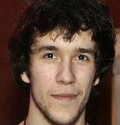
\includegraphics[width=0.8\linewidth]{60}
  \caption{Bruno Ferreira  }
\end{subfigure}%
\begin{subfigure}{.33\textwidth}
  \centering
  
\includegraphics[width=0.8\linewidth]{107}
  \caption{Cláudia Oliveira}
\end{subfigure}%
\begin{subfigure}{.33\textwidth}
  \centering
  
\includegraphics[width=0.8\linewidth]{93}
  \caption{Vanessa Campos}
\end{subfigure}%
\end{figure}


\end{document}